\chapter{Background}

% WHAT IS A COMPILER 

To allow for a higher abstraction and higher thinking when resoning about 
algorithms new language has be developed. To be able to run these new languages
compilers has been built to "translate" the code down to machine code to run 
directly or to a lower level language to make use of their compiler. 

% HOW IS A COMPILER BUILT 

When building a compiler it can be resembled to a pipe where text flows through 
while transformed into different representations and in the end outputted
to runnable code to either run on the computer itself or on a virtual machine
that emulates a computer.

Now is Hopper really a transpiler or a translating compiler. Instead of 
outputting runnable code it outputs other code that is interpreted and compiled
by the Erlang compiler, erlc. With this the project could very much be 
simplified (ref to read more in discussion).

% PIPELINE FIGURE

\begin{figure}[h!]
\label{fig:pipeline}
\centering
  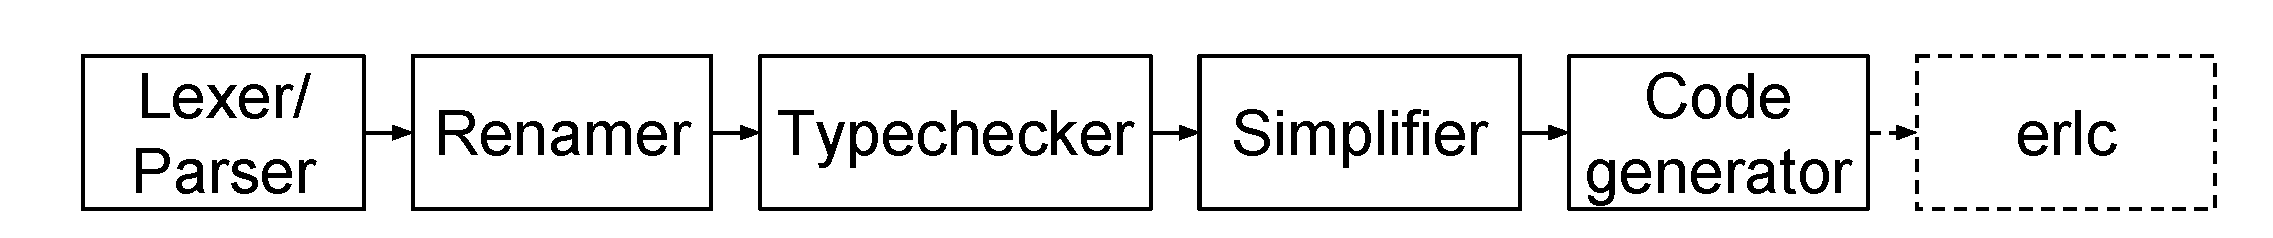
\includegraphics[width=0.6\pdfpagewidth]{figure/pipeline}}
\end{figure}

% HOW IS HOPPER BUILT

As seen in figure~\ref{fig:pipeline} the Hopper language has five steps in its 
pipeline before it turns it over to the Erlang compiler. Each step work on the 
source code representation in a uniqe way. The steps can be summerized as
follows. The lexer and parser reads in text files and converts them to an 
abstract representation, the renamer simplify this representation for that 
typechecker whos job it is to control the types of thefunctions. Second to last 
there is another simplifying step before the code generator who writes the
assembly code that is run on the BEAM VM.

% OTHER SECTIONS

\section{Parsing source code} \label{sec:bnfc}

\todo{Assigned David}


A programming language is similar to a natural language in that it is described by a grammar. Programming languages are however different in that they are built from their grammar and are thus unambiguous.
The grammar describes ways in which the smaller pieces of the language can be put together to form bigger ones, often with more meaning. 

From this grammar a lexer is produced. The lexers job is to match all words in the source code to tokens in the grammar. For example in english the word 'boat' would match a noun token. This list of tokens is combined with a parser to make expressions or sentences. To make the language as expressive as possible one build up bigger expressions out of smaller expressions. This will create a tree structure that will be easier to work with. 

To save a lot of work, the lexer and parser can be automatically generated from a grammar written in \gls{bnf} using a tool called the \gls{bnfc} \cite{bnfc}, or BNFC for short. This tool is developed at Chalmers and used in earlier courses, meaning that multiple group members were already familiar with it.
\section{Renaming and simplifying}

\todo{Assigned DAvid}

While BNFC is a great tool to create a parse tree from raw text the resulting 
tree structure is very verbose with a lot of constructors. To simplify this a
renamer step is introduced in the pipeline. This step converts the parse tree
to our minimally designed \acrlong{ast} or \acrshort{ast} for short. 

% TODO I want these beside each other and a arrow in between
\begin{table}
\begin{lstlisting} 
f = if a                      f = case a of
      then b        =>              True  -> b
      else c                        False -> c
\end{lstlisting}
\caption{Simple transformation to a more general form}
\label{lst:renamer1}
\end{table}

In this step a few grammar rules could be translated to more general expressions
to simplify the AST and reduce the number of cases the typechecker need to cover, see
table \ref{lst:renamer1}.

The other part of the renamer module is to annotate the functions to where they
where exported from...


